\newcommand{\FigQueryTime}{
\begin{figure}
    \centering
    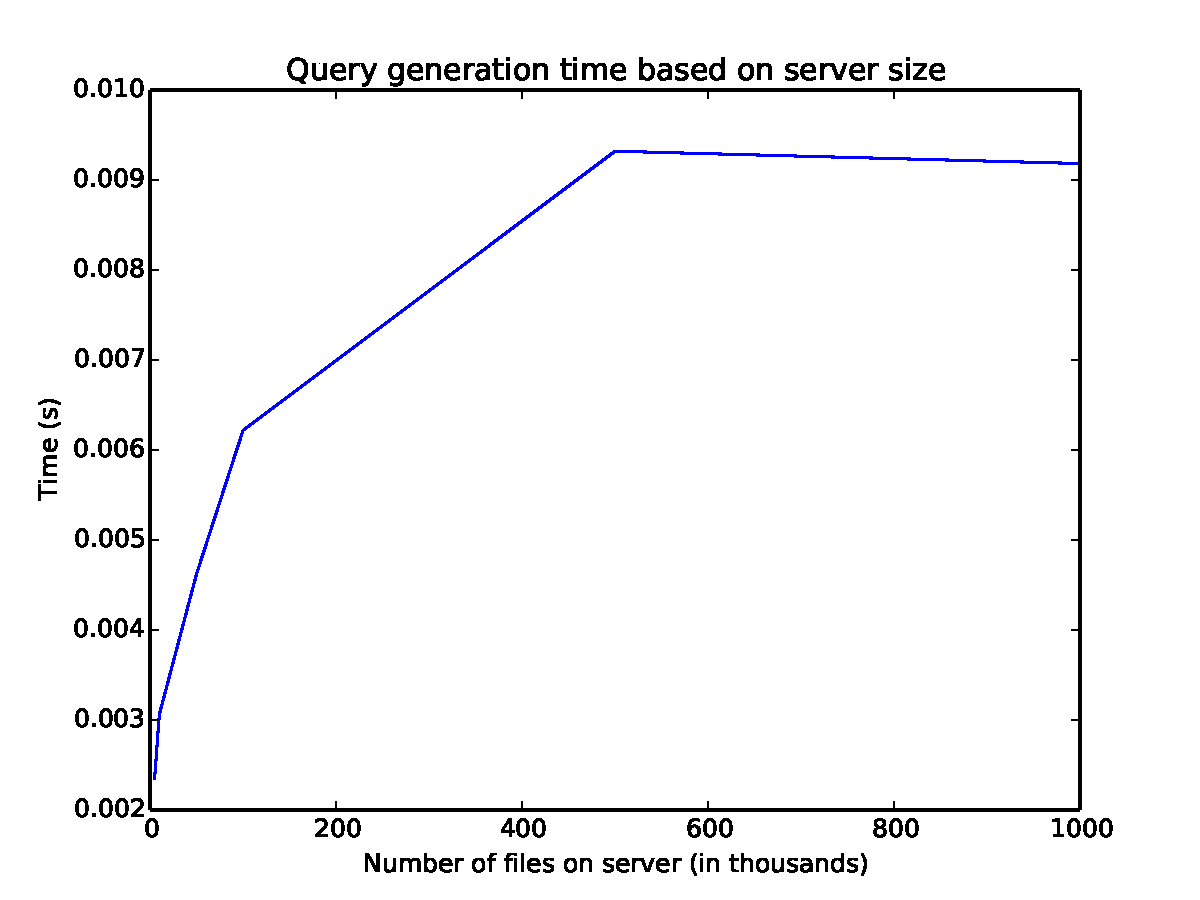
\includegraphics[width=\linewidth]{figs/QueryGenTime}
    \caption{The amount of time taken for the client to generate enough
    queries to privately ask the server for a single file.}
    \label{fig:querygentime}
\end{figure}
}

\newcommand{\FigReplyTime}{
\begin{figure}
    \centering
    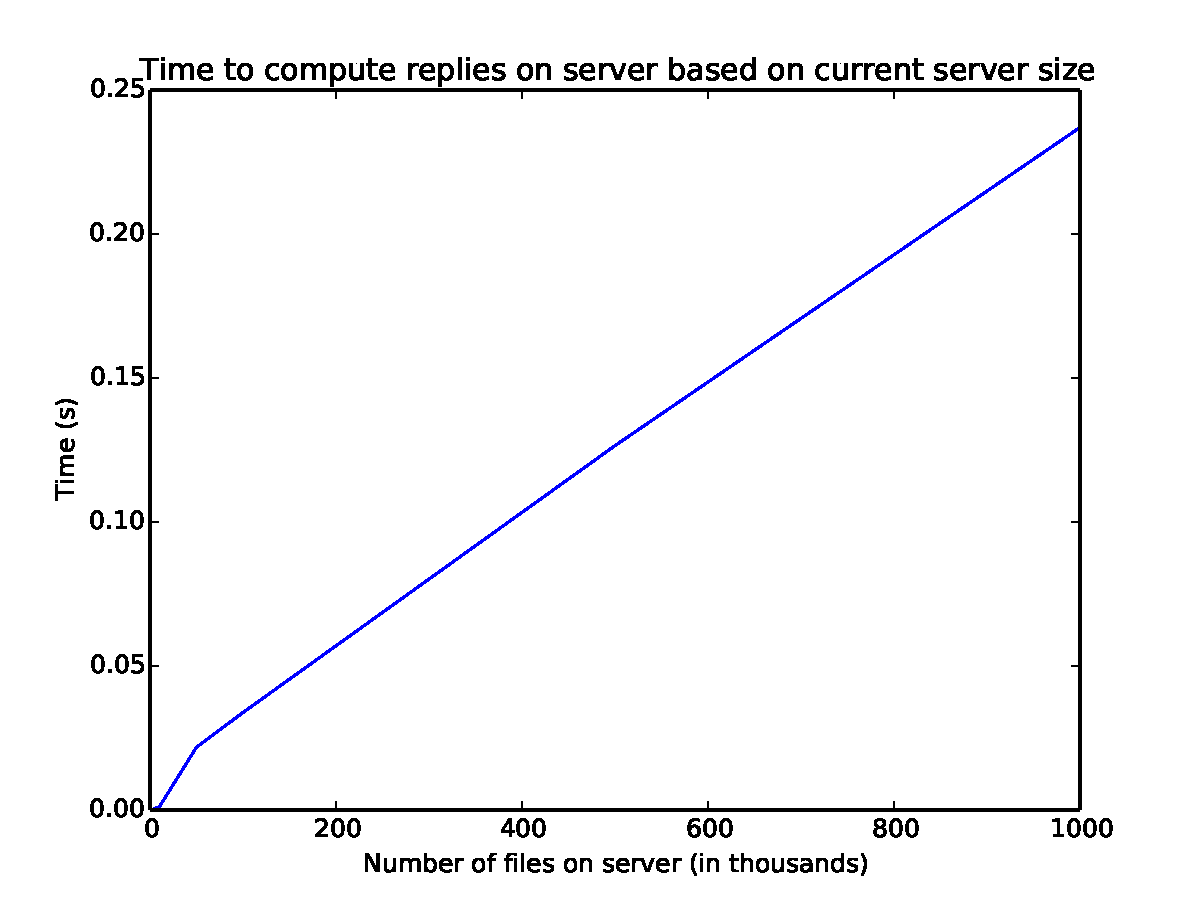
\includegraphics[width=\linewidth]{figs/ReplyTime}
    \caption{Amount of time taken for server to compute the replies to queries
    sent by client}
    \label{fig:replyTime}
\end{figure}
}

\newcommand{\FigExtractTime}{
\begin{figure}
    \centering
    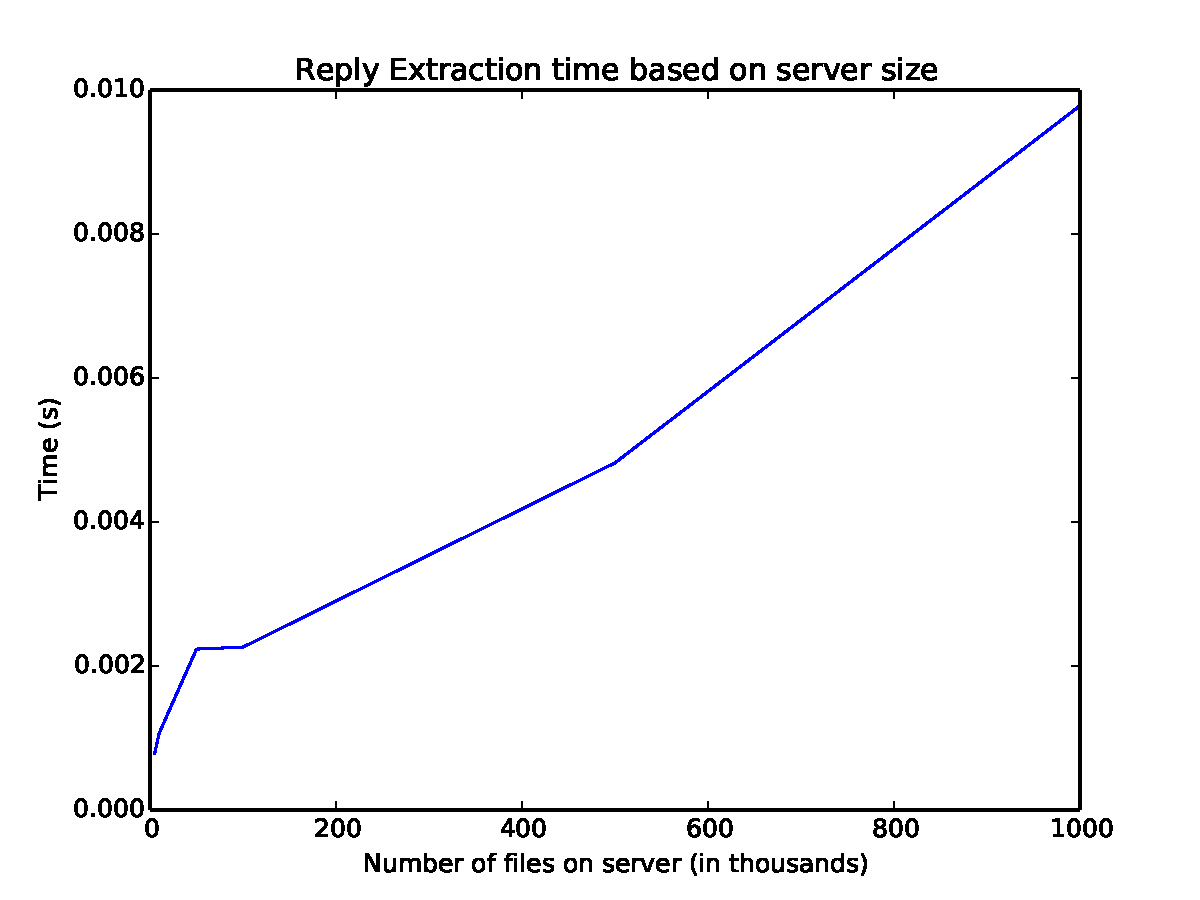
\includegraphics[width=\linewidth]{figs/ReplyExtractTime}
    \caption{Amount of time taken for the client to extract response
    from replies
    provided by the server}
    \label{fig:replyextracttime}
\end{figure}
}

\newcommand{\FigAllTimes}{
\begin{figure}[ht]
    \centering
    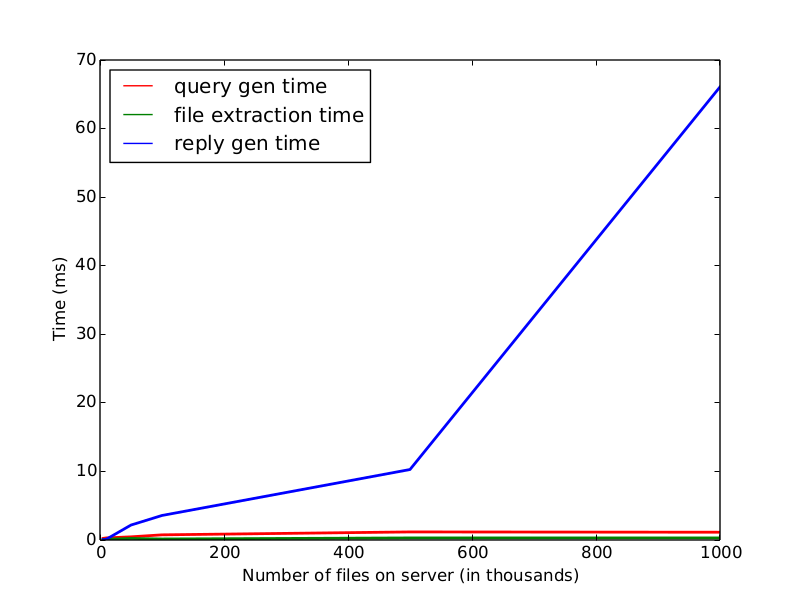
\includegraphics[width=0.7\linewidth]{figs/QueryReplyExtractOneAxisNet}
    \caption{Amount of time taken for the actions necessary for our tool to
    work. The time taken for the client to generate queries, and to extract the
    response from the server replies is very minimal compared to the amount of
    time that is spent by the server generating the replies to send back to the
    server. This time however can be decreased by using servers with hardware
    specifically designed to do these computations.}
    \label{fig:queryreplyextracttime}
\end{figure}
}

\newcommand{\FigPIR}{
\begin{figure}[ht]
    \centering
    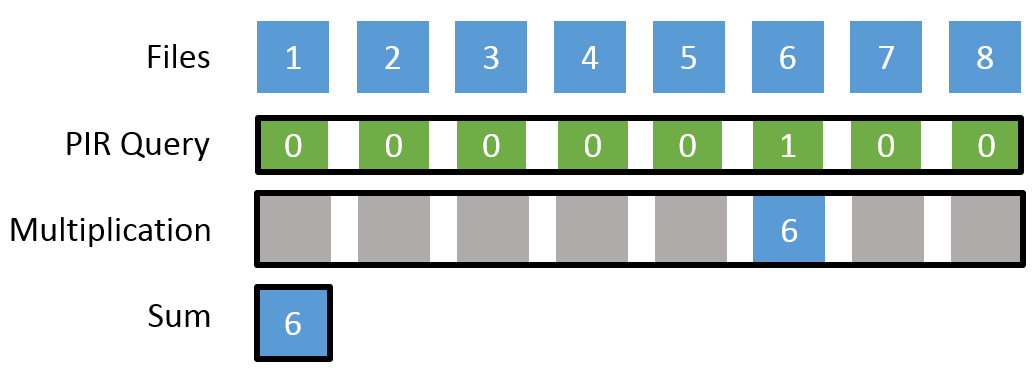
\includegraphics[width=.8\linewidth]{figs/pir-basic.png}
    \caption{\textbf{Vector-Matrix PIR}\,---\, Private Information Retrieval
    involves a client making
    a query against a database. In Vector-Matrix PIR the client encrypts a vector of  query elements and the server then multiplies the query elements
    against the database blocks homomorphically, using homomorphic addition to produce a single sum.
    This results in an encrypted value corresponding to the element where the client encrypted 1
    (instead of 0), which is sent back to the client for decryption.}
    \label{fig:pir}
\end{figure}
}


\newcommand{\FigTicket}{
\begin{figure}[ht]
    \centering
    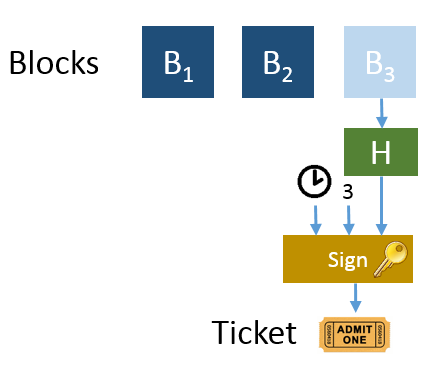
\includegraphics[width=.5\linewidth]{figs/ticket-small.png}
    \caption{\textbf{Ticket Creation}\,---\, When a file is uploaded, the server produces
            a signed ticket that commits the server to storing the block of data. The server
            signs a timestamp, the index where the data is stored, and a hash of the data, and
            returns this to the client for local storage.}
    \label{fig:ticket}
\end{figure}
}


\newcommand{\FigProof}{
\begin{figure}[ht]
    \centering
    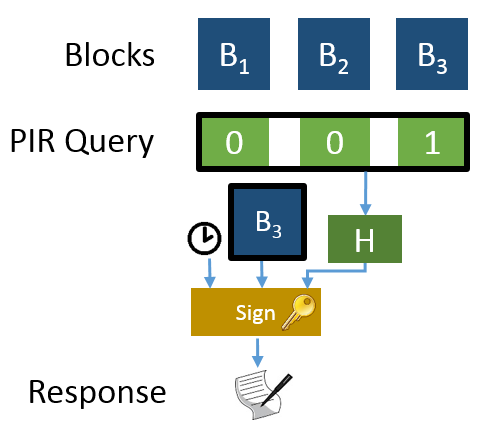
\includegraphics[width=.5\linewidth]{figs/query-small.png}
    \caption{\textbf{Proof of Censorship}\,---\, To verify a file is still in place, a client
            constructs a PIR query for its block. The
            server, without knowing which block was requested, signs the encrypted PIR query and the
            response it produces. The client decrypts the response, and can verify the data is
            correct. If it is not, the client can combine the signed response, the parameters it used
            to generate the PIR query, and the original
    ticket for this file to produce a stand-alone proof-of-censorship that can be verified by a third
    party.}
    \label{fig:proof}
\end{figure}
}


\newcommand{\TabSizes}{
\begin{table}
\centering
\begin{tabular}{l|c|c|c}
            \hline
            & Size & Generation time  (std-dev)& Validation time (std-dev)\\
            \hline

        Ticket & 120 bytes & 334 {\textmu}s (0.53) & 381 {\textmu}s (4.61)\\
        Query  & 3.8 Mbytes & 28 ms (0.44) & n/a \\
        Reply/Proof\ \  & 2.0 Mbytes & 2.8 s (0.19) & 52 ms (0.54) \\
\end{tabular}
\caption{\textbf{Ticket and Proof Size}\,---\, We implemented a prototype of our proof-of-censorship
system, simulating a database of 1~million 256-byte messages. We are able to
keep a constant size of our proof at 2 MB. This allows clients that receive a
proof of censorship to be able to easily distribute it.}
\label{tab:size}
\end{table}
}

\newcommand{\TabNumQueries}{
\begin{table}[ht]
\centering
\begin{tabular}{c|c|c|c|c|c|c|c|c}
        \hline
        Number of files    & 5k     & 10k    & 50k     & 100k   & 500k   & 1M 
        & 10M  & 100M\\
        \hline

        Recursion depth    &  1     &  1     &  2      &  2     &   2    &   3 
        & 3  & 3\\
        Aggregation value  & 300    & 420    & 96      & 64     & 126    &  16
        & 16 & 15\\

        Query size (MBytes)    & 0.53 & 0.75 & 1.44 & 2.5  & 3.9  & 3.8 & 8.0  &
        17.7 \\

        Reply size (MBytes)    & 0.56 & 0.78 & 1.44  & 1.0  & 2.0  & 2.0
         & 2.0  & 2.4 \\
\end{tabular}
\caption{\textbf{Small File Scaling}\,---\, We measured query and response sizes
    generated for several different database sizes with 256~byte files to determine
    how the system scales for a Twitter-like content server. We find that even at millions
    of files, the system remains
    relatively practical: an 8~MByte query and 2~MByte response are needed to select
    a single file privately (with accompanying proof of censorship) from 10~million files.}
\label{tab:numQueries}
\end{table}
}

\newcommand{\TabNumMBQueries}{
\begin{table}[ht]
\centering
\begin{tabular}{c|c|c|c|c|c|c|c|c}
        \hline
        Number of files    & 5k      & 10k    & 50k     & 100k   & 500k   & 1M 
        & 10M  & 100M\\
        \hline

        Recursion depth    &  2      &  2     &  2      &  2     &   2    &   2 
        & 3  & 3\\
        Aggregation value  & 1       & 1      & 1      & 1      & 1       &  1
        & 1 & 1\\

        Query size (MBytes)    & 17.8  & 25.0 & 14.0 & 19.8 & 44.2 &
        62.5 & 121.3 & 174.1 \\

        Reply size (MBytes)    & 32.8  & 32.8  & 73.1  & 73.1  & 83.7  &
        83.7  & 138.4  & 199.4 \\
        % Bits of Security & 209 & 209 & 248 & 248 & 248 & 248 & 90 & 209\\
        % Polynomial Degree & 4096 & 4096 & 2048 & 2048 & 2048 & 2048 & 4096 &
        % 4096\\
        % Modulus Bits & 60 & 120& 60 & 60 & 60 & 60 & 180 & 120\\
\end{tabular}
\caption{\textbf{Large file scaling}\,---\, We also measured query and response sizes
        assuming 1~MByte files, to approximate our system being applied to an image or video-streaming
        content server. The XPIR optimizer chooses different security,
        polynomial and modulus parameters for each database size for 1~MByte
        files, due to it attempting to limit the amount of data the client
        has to send and receive over the network. While the parameters that
        are chosen are not always the most secure or privacy preserving,
        these parameters do result in the least amount of bandwidth
        necessary for clients to use. Additionally, while overheads are low,
        even with only 50
        thousand files
        in a database, responses are 73~MBytes for a single megabyte file, likely making application of
        proof of censorship impractical to video streaming content providers.}
\label{tab:numMBQueries}
\end{table}
}
